%!TEX root = ../paper.tex

\section{Implementation}
\label{sec:implementation}
In the following our approach to determine different writing style groups using k-means clustering and assigning a new blog posts to one of those groups is shown.


% TODO Details zu Features: Ein zwei genauer erklären
% Quellen der Features angeben.
% Woher kommen die function word, etc. listen?

% TODO Welche Libraries, welche Parameter wurden genutzt?
% Standford Tagger, LibSVM, Langauge Detection


% Erklärung von K-nearest neighbor etc. hier


\subsection{Features}
\label{sec:impl_features}

\begin{savenotes}


In Table~\ref{tab:featureTable} we describe all the features we used along with their respective individual feature count.
One of the features we utilized, the \textit{function word} feature might appear to clash with our desire to create a topic-independent algorithm, which does not use a \textit{bag of words} model.
However, function words are words with little or no lexical meaning, mainly used to create the grammatical structure of a sentence.
Thus, they are actually topic-independent and the frequency of their usage has been successfully utilized to identify authors~\cite{mosteller1962applied}.
We also tried to achieve topic-independence for our list of common abbreviations, which we used in the same way.
The full list of function words and abbreviations we used for German and English can be found in Appendix~\ref{sec:app_function_words} and~\ref{sec:app_abbreviations}).


\begin{table}[ht!]
    \begin{center}
    \begin{tabular}{p{2.6cm}|p{6cm}|p{1.2cm}|p{1.2cm}}
    Feature                 & Description                                                               & Count             & Source\\ \hline \hline
    Blank line               & 1 divided by number of blank lines in the text                            & 1                 & \cite{de2001mining}\\ \hline
    Capital letter           & Capital letters divided by all letters                                    & 1                 & \cite{argamon2003style} \cite{de2001mining}\\ \hline
    Emoticon                & Boolean value for occurrence of known emoticons                           & 9                 & original\\ \hline
    Function word            & Fraction of words that are a known function word.                         & 280[DE] 280[EN]   & \cite{argamon2003style} \cite{de2001mining} \cite{madigan2005author} \cite{narayanan2012feasibility}\\ \hline
    Abbreviations           & Words that are a known abbreviation                                       & 53[DE] 53[EN]     & original\\ \hline
    Number character         & Fraction of characters that are numeric characters (0-9)                  & 1                 & \cite{narayanan2012feasibility}\\ \hline
    Paragraph               & Number of paragraphs divided by average paragraph length                  & 1                 & \cite{argamon2003style}\\ \hline
    PoSTag                  & Fraction of words that have a certain part-of-speech tag. To identify the part-of-speech tags we used the Standford Tagger\footnote{\url{http://nlp.stanford.edu/software/tagger.shtml}}
                                                                                                        & 55[DE] 46[EN]     & \cite{madigan2005author}\\ \hline
    Post length              & 1 divided by the number of characters                                     & 1                 & \cite{narayanan2012feasibility}\\ \hline
    Prefix/suffix            & 2-letter prefixes/suffixes divided by total number of prefixes/suffixes   & 676               & \cite{madigan2005author}\\ \hline
    Punctuation character   & Fraction of characters that are a known punctuation character             & 11                & \cite{madigan2005author} \cite{narayanan2012feasibility}\\ \hline
    Sentence length          & 1 divided by the average sentence length                                  & 1                 & \cite{de2001mining}\\ \hline
    Single occurring word    & Words that occur only once divided by all distinct words                  & 1                 & \cite{madigan2005author} \cite{narayanan2012feasibility}\\ \hline
    Upper case           & Words that are fully in upper case divided by all words                   & 1                 & original\\ \hline
    Word frequency           & 1 divided by the average number of occurrences per word                   & 1                 & \cite{madigan2005author} \cite{narayanan2012feasibility}\\ \hline
    Word length              & 1 divided by the average word length                                      & 1                 & \cite{argamon2003style} \cite{narayanan2012feasibility}\\
    \end{tabular}
    \end{center}
    \caption{Implemented features with descriptions, the count of individual features they contribute to the feature vector, and papers they have previously been utilized in.}
    \label{tab:featureTable}
\end{table}


One of the features we utilized, the function word feature, might appear to clash with our desire to create a topic-independent algorithm, which does not use a bag of words model.
However, function words are words with little or no lexical meaning, mainly used to create the grammatical structure of a sentence.
Thus, they are actually topic-independent and the frequency of their usage has been successfully used to identify authors~\cite{mosteller1962applied}.
We also tried to achieve topic-independence for our list of common abbreviations, which we used in the same way.
The full list of function words and abbreviations we used for German and English can be found in Appendix~\ref{sec:app_function_words} and~\ref{sec:app_abbreviations}.

\end{savenotes}

After evaluating our features (see Section~\ref{sec:evaluation_clustering}) we decided to drop the \textit{prefix/suffix} and \textit{PoSTag} features and keep all others.




\subsection{Clustering}
\label{sec:impl_clustering}

For our implementation we used the \textit{k-means} algorithm offered by Mahout\footnote{\url{https://mahout.apache.org/}}, which can be executed efficiently among a cluster with a large amount of data~\cite{esteves2011k}.


\textit{K-means} creates $k$ clusters from $n$ vectors by randomly selecting $k$ points from the vector space as cluster centroids.
Then, each vector or point is assigned to its nearest cluster centroid according to its \textit{Euclidean} distance to those centroids.
Afterwards, the cluster centroids are repositioned to the center of all vectors/points, which were assigned to them.
These last two steps are repeated until the cluster centroids converge.
The resulting assignment of the vectors (and thus their corresponding blog posts) to the clusters is the same as the final assignment performed by the \textit{k-means} algorithm.


Using our small data set we set $k$ to 6, the number of authors.
Under the assumption that each author has an individual writing style and that this writing style is not changing over time, an author should obtain their own cluster containing only blog posts written by him.
In this way, we could evaluate our \textit{k-means} algorithm (see Section~\ref{sec:evaluation_clustering}).



\subsection{Classification}
\label{sec:impl_classification}


The first naive idea, which assigns a cluster to a blog post, is to calculate the euclidean distance from the blog post to the central points of each cluster.
The resulting cluster would then be the one with the lowest distance.
While this method is computationally simple and fast, it might not provide the best possible results.
Therefore we looked at more sophisticated approaches that were used for similar problems before.
We applied two of those methods, a k-Nearest neighbor algorithm~\cite{peterson2009k} and a Support Vector Machine~\cite{kolari2006svms}.
The training data for these algorithms is based on the clustering results, as described in Section~\ref{sec:classification}.


\subsubsection{k-Nearest Neighbor}
\label{sec:k_nearest_neighbor}


The k-Nearest Neighbor algorithm selects the $k$ vectors from the training data which are closest to the feature vector of the new blog post.
Then it returns the cluster that is prevalent amongst these neighbors as a result.
For example consider the scenario depicted in Figure~\ref{fig:naive}.
The naive method of calculating the euclidean distance between the cluster center and the feature vector of the new blog post would have cluster 1 as a result.
However the k-Nearest Neighbor algorithm with, for example $k=5$, returns cluster 2, because four out of the five closest neighbors belong to cluster 2.
Intuitively, this appears like the better solution because the feature vector of the new blog post seems to be naturally belonging to cluster two.


\begin{figure}[h]
    \centering
    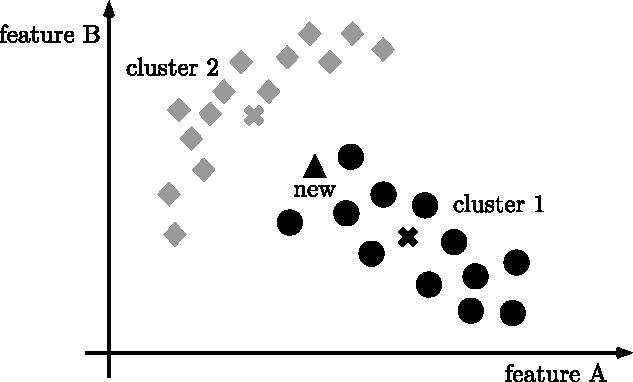
\includegraphics[width=0.6\textwidth]{images/naive.pdf}
    \caption{The naive approach, which calculates the euclidean distance to the center of the cluster, would put the new blog post into cluster 1. The k-Nearest Neighbor algorithm would return cluster 2 as a result.}
    \label{fig:naive}
\end{figure}


\subsubsection{Support Vector Machine}
\label{sec:support_vector_machine}


A Support Vector Machine creates a model to distinguish between the different clusters of the training data by calculating borders between them.
These borders can be thought of as functions in the same vector space as the feature vectors.
If the Support Vector Machine uses a linear model, this might look like Figure~\ref{fig:svm}, represented in a two-dimensional graph.
Both, the dotted and the dashed line serve as examples for a possible border, but the Support Vector Machine should usually tend to use the model with more distance to all feature vectors.
In this case, the dashed line would more accurately divide cluster 1 and 2.


We used the support vector machine implementation LIBSVM\footnote{\url{http://www.csie.ntu.edu.tw/~cjlin/libsvm/}}, as described by Fan et al.~\cite{fan2005working}.
We followed the configuration procedure proposed by Hsu et al.~\cite{hsu2003practical}.
In the end we used the default configuration of type C-SVC and a radial basis function kernel for the support vector machine.
The only parameter we adapted was $c=1000$, which was done using cross-validation, as recommended by Hsu et al. to prevent overfitting on our data set.


\begin{figure}[h]
    \centering
    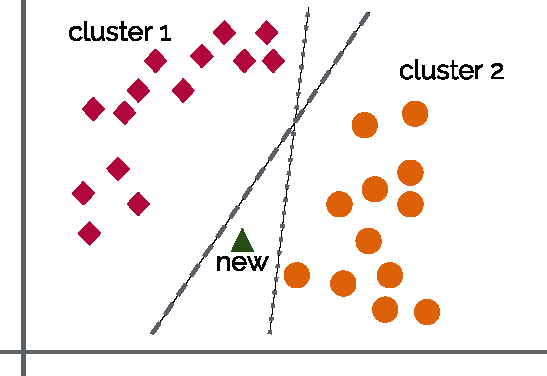
\includegraphics[width=0.6\textwidth]{images/svm.pdf}
    \caption{Two differently configured Support Vector Machines might provide the two different lines as borders between the different clusters. The dotted line would result in the blog post belonging to cluster 1, while the dashed line would return cluster 2 as a result.}
    \label{fig:svm}
\end{figure}
